\chapter{Estimador de odometría Visual e inercial}

\section{Arquitectura}

El algoritmo de odometría visual-inercial implementado sigue una formulación robocéntrica basada conceptualmente en 
R-VIO2~\cite{huai2022square}. En este enfoque, la estimación no se realiza directamente respecto a un marco global fijo, 
sino respecto a un marco local asociado al movimiento del propio sensor. Esta elección permite mantener una ventana 
deslizante de estados relativos y actualizar el sistema mediante una matriz de información en forma \textit{square-root}. 
Aunque el diseño general se inspira en dicho trabajo, la implementación utilizada en este proyecto ha sido desarrollada 
de forma propia. La arquitectura del sistema se muestra en la Figura~\ref{fig:vio_arq}.


\begin{figure}[H]
    \ffigbox[\FBwidth] {
        \caption[Arquitectura del sistema de odometría visual-inercial.]{Arquitectura del sistema de odometría visual-inercial.}
        \label{fig:vio_arq}
    }
    {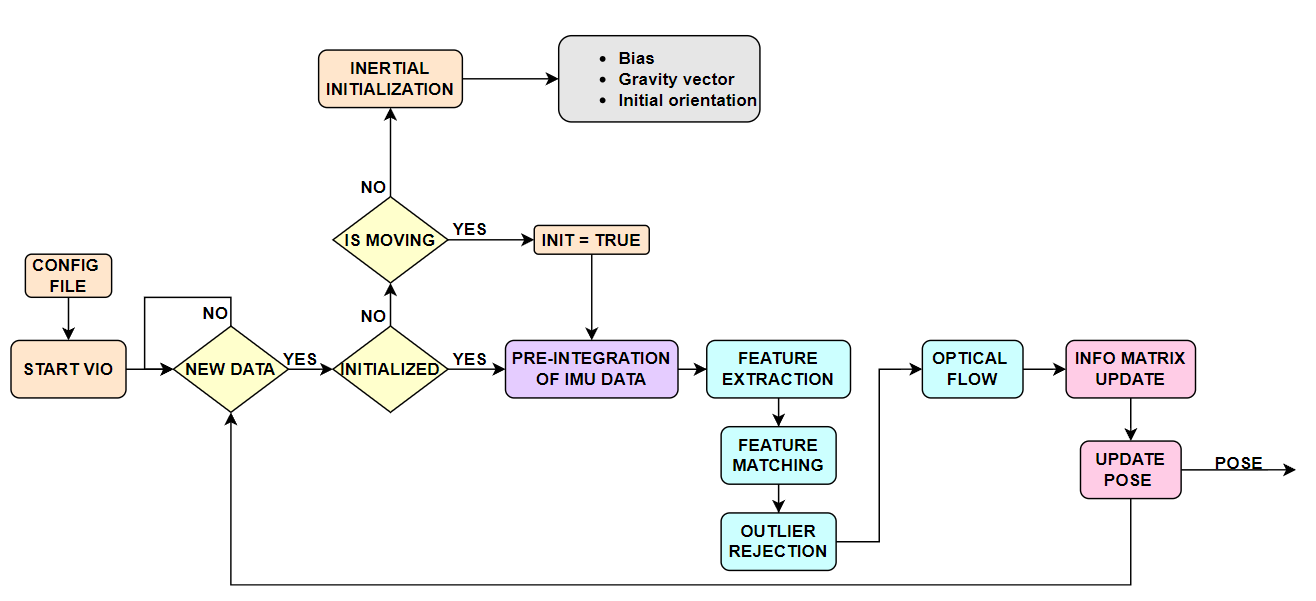
\includegraphics[scale=0.38]{images/vio_arquitecture.png}}
\end{figure}



El flujo principal del algoritmo se puede resumir en los siguientes pasos:

\begin{enumerate}[nosep]
    \item Se recibe un paquete, compuesto por una imagen RGB y una secuencia de medidas IMU sincronizadas con el intervalo de dos imágenes consecutivas.
    \item Si el sistema aún no ha sido inicializado, se estima la dirección de la gravedad y los sesgos iniciales de la IMU a partir de un intervalo en reposo.
    \item Se propaga el estado mediante pre-integracion inercial, generando un nuevo factor IMU y actualizando la matriz de información \textit{square-root}.
    \item Se predice la pose de la cámara a partir del estado propagado.
    \item Se realiza el seguimiento visual de características mediante flujo óptico KLT y se rechazan correspondencias erróneas mediante RANSAC.
    \item Se triangulan nuevas features usando parametrización de profundidad inversa.
    \item Se construyen los factores visuales y se incorporan al sistema mediante actualizaciones QR.
    \item Se aplica la corrección estimada al estado y se realiza la composición robocéntrica, cambiando el marco local de referencia al instante actual.
\end{enumerate}

\section{Inicialización del sistema}

La inicialización del sistema tiene como objetivo estimar las condiciones iniciales necesarias para comenzar la odometría visual-inercial. En concreto, se calculan tres magnitudes principales: la dirección inicial de la gravedad, el sesgo inicial del giróscopo y el sesgo inicial del acelerómetro. Estas variables son fundamentales, ya que el estimador necesita partir de una orientación coherente y de unas medidas inerciales corregidas antes de iniciar la propagación del estado.

El procedimiento se basa en detectar un intervalo inicial en el que la plataforma permanezca aproximadamente en reposo. Para ello, se analizan las muestras IMU recibidas y se estima el movimiento angular y el desplazamiento aproximado durante dicho intervalo. En primer lugar, se elimina de forma aproximada la componente de la gravedad de la aceleración medida y se acumulan las variaciones de orientación, velocidad y posición:

\begin{equation}
\begin{aligned}
    \Delta \boldsymbol{\theta}
    &=
    \sum_i
    \boldsymbol{\omega}_i \Delta t_i,
    \\
    \Delta \mathbf{v}
    &=
    \sum_i
    \mathbf{a}_i \Delta t_i,
    \\
    \Delta \mathbf{p}
    &=
    \sum_i
    \left(
        \Delta \mathbf{v}_i \Delta t_i
        +
        \frac{1}{2}
        \mathbf{a}_i \Delta t_i^2
    \right).
\end{aligned}
\end{equation}

Si la variación angular y el desplazamiento estimado son inferiores a los umbrales configurados, el sistema considera que el UAV todavía no se ha movido. En ese caso, las medidas de acelerómetro y giróscopo se acumulan para calcular una media más robusta. Además, se almacena la última imagen recibida, que será utilizada posteriormente para inicializar el sistema de seguimiento visual.

Cuando se detecta movimiento, el sistema deja de acumular medidas y calcula las condiciones iniciales. Si se han acumulado suficientes muestras, se calcula la media de las medidas inerciales. A partir de esta media se estima la dirección de la gravedad, el sesgo del giróscopo y el sesgo del acelerómetro:

\begin{equation}
\begin{aligned}
    \mathbf{g}
    &=
    \frac{\bar{\mathbf{a}}}
    {\left\|\bar{\mathbf{a}}\right\|},
    \\
    \mathbf{b}_g
    &=
    \bar{\boldsymbol{\omega}},
    \\
    \mathbf{b}_a
    &=
    \bar{\mathbf{a}}
    -
    g_0 \mathbf{g}.
\end{aligned}
\end{equation}

donde $\bar{\boldsymbol{\omega}}$ es la media de las velocidades angulares, $\bar{\mathbf{a}}$ es la media de las aceleraciones medidas, $g_0$ es el módulo de la gravedad y $\mathbf{g}$ es la dirección estimada de la gravedad. En caso de que la plataforma comience ya en movimiento y no exista un intervalo inicial en reposo, el sistema utiliza la última muestra disponible como estimación inicial, aunque en este caso los sesgos se inicializan a cero.

Una vez calculadas estas magnitudes, se inicializa el vector de estado local del estimador. Este vector contiene la orientación y posición iniciales, la dirección de la gravedad, la calibración extrínseca cámara-IMU, el desfase temporal entre sensores, la velocidad inicial y los sesgos de la IMU:

\begin{equation}
    \mathbf{x}_0
    =
    \left[
        \mathbf{q}_G,
        \mathbf{p}_G,
        \mathbf{g},
        \mathbf{q}_{CI},
        \mathbf{t}_{CI},
        t_d,
        \mathbf{v},
        \mathbf{b}_g,
        \mathbf{b}_a
    \right].
\end{equation}


La calibración extrínseca entre la cámara y la IMU se inicializa con los valores disponibles en la configuración, es decir, con la rotación $\mathbf{q}_{CI}$ y la traslación $\mathbf{t}_{CI}$. El desfase temporal inicial entre cámara e IMU se establece a cero. La velocidad inicial también se considera nula, mientras que los sesgos se inicializan con los valores estimados durante el intervalo en reposo.

Además del vector de estado, se inicializa la matriz de información local del estimador. Esta matriz introduce la confianza inicial sobre cada una de las variables del estado. Las variables conocidas con mayor precisión, como la pose inicial, se inicializan con una incertidumbre baja. En cambio, los parámetros de calibración cámara-IMU y el desfase temporal se inicializan con una incertidumbre dependiente de si existe o no una calibración previa conocida. Si dicha calibración está disponible, se asigna una confianza mayor; en caso contrario, se permite que el estimador corrija estos parámetros con mayor libertad durante la navegación.

Finalmente, se inicializa el módulo de seguimiento visual utilizando la última imagen almacenada durante la fase de reposo. Con ello se detectan las primeras características visuales y se fija la primera pose válida del sistema. A partir de este momento, el estimador queda marcado como inicializado y puede comenzar el proceso normal de propagación inercial, seguimiento visual y actualización del estado.

\section{Preintegración inercial}

La preintegración inercial permite condensar un conjunto de medidas IMU de alta frecuencia, tomadas entre dos fotogramas 
consecutivos, en una única restricción de movimiento. Esta técnica es especialmente útil en sistemas visual-inerciales, ya 
que evita tener que actualizar el estado completo del estimador con cada muestra de la IMU. En su lugar, las medidas 
inerciales se acumulan localmente y se incorporan posteriormente al sistema como un único factor entre dos instantes 
visuales~\cite{morris2024imu_preintegration}.

El punto de partida es el modelo de medida de una IMU. El giróscopo mide la velocidad angular afectada por un sesgo y por 
ruido blanco:

\begin{equation}
    \tilde{\boldsymbol{\omega}}_k
    =
    \boldsymbol{\omega}_k
    +
    \mathbf{b}_{g,k}
    +
    \boldsymbol{\eta}_{g,k},
\end{equation}

mientras que el acelerómetro mide la fuerza específica, también afectada por sesgo y ruido:

\begin{equation}
    \tilde{\mathbf{a}}_k
    =
    \mathbf{R}_{WB,k}^{T}
    \left(
        \mathbf{a}_{W,k}
        -
        \mathbf{g}_{W}
    \right)
    +
    \mathbf{b}_{a,k}
    +
    \boldsymbol{\eta}_{a,k}.
\end{equation}

En estas expresiones, $\tilde{\boldsymbol{\omega}}_k$ y $\tilde{\mathbf{a}}_k$ son las medidas proporcionadas por la IMU, $\mathbf{b}_{g,k}$ y $\mathbf{b}_{a,k}$ son los sesgos del giróscopo y del acelerómetro, $\boldsymbol{\eta}_{g,k}$ y $\boldsymbol{\eta}_{a,k}$ representan el ruido de medida, $\mathbf{R}_{WB,k}$ es la rotación del cuerpo respecto al sistema global y $\mathbf{g}_{W}$ es el vector de gravedad.

Corrigiendo las medidas con los sesgos estimados, se obtiene

\begin{equation}
    \boldsymbol{\omega}_k
    =
    \tilde{\boldsymbol{\omega}}_k
    -
    \mathbf{b}_{g,k},
    \qquad
    \mathbf{a}_k
    =
    \tilde{\mathbf{a}}_k
    -
    \mathbf{b}_{a,k}.
\end{equation}

A partir de estas medidas corregidas, el modelo cinemático continuo de la IMU puede escribirse como

\begin{equation}
\begin{aligned}
    \dot{\mathbf{R}}_{WB}
    &=
    \mathbf{R}_{WB}
    \left[
        \boldsymbol{\omega}
    \right]_{\times},
    \\
    \dot{\mathbf{p}}_{W}
    &=
    \mathbf{v}_{W},
    \\
    \dot{\mathbf{v}}_{W}
    &=
    \mathbf{R}_{WB}
    \mathbf{a}
    +
    \mathbf{g}_{W},
\end{aligned}
\end{equation}

donde $\left[\cdot\right]_{\times}$ representa la matriz antisimétrica asociada al producto vectorial.

En una integración directa, cada muestra de la IMU se utilizaría para propagar orientación, posición y velocidad en el sistema global. Sin embargo, esto obliga a trabajar continuamente con el estado completo del estimador y con la gravedad expresada en el marco global. La idea principal de la preintegración consiste en acumular las medidas IMU en un marco local asociado al instante inicial del intervalo. De este modo, se calculan tres incrementos relativos:

\begin{equation}
    \Delta \mathbf{R}_{ij},
    \qquad
    \Delta \mathbf{p}_{ij},
    \qquad
    \Delta \mathbf{v}_{ij},
\end{equation}

que representan, respectivamente, el incremento de rotación, posición y velocidad entre los instantes $i$ y $j$.

Al inicio de cada intervalo de preintegración se inicializan los incrementos como

\begin{equation}
\begin{aligned}
    \Delta \mathbf{R}_{ij}
    &=
    \mathbf{I},
    \\
    \Delta \mathbf{p}_{ij}
    &=
    \mathbf{0},
    \\
    \Delta \mathbf{v}_{ij}
    &=
    \mathbf{0},
    \\
    \Delta t_{ij}
    &=
    0.
\end{aligned}
\end{equation}

Para cada muestra IMU recibida dentro del intervalo, con paso temporal $\delta t_k$, se calculan los incrementos elementales:

\begin{equation}
\begin{aligned}
    \delta \mathbf{R}_{k}
    &=
    \operatorname{Exp}
    \left(
        \left[
            \boldsymbol{\omega}_k
        \right]_{\times}
        \delta t_k
    \right),
    \\
    \delta \mathbf{v}_{k}
    &=
    \mathbf{a}_k
    \delta t_k,
    \\
    \delta \mathbf{p}_{k}
    &=
    \frac{1}{2}
    \mathbf{a}_k
    \delta t_k^2.
\end{aligned}
\end{equation}

Estos incrementos se acumulan de forma recursiva mediante

\begin{equation}
\begin{aligned}
    \Delta \mathbf{p}_{ij}
    &\leftarrow
    \Delta \mathbf{p}_{ij}
    +
    \Delta \mathbf{v}_{ij}
    \delta t_k
    +
    \Delta \mathbf{R}_{ij}
    \delta \mathbf{p}_{k},
    \\
    \Delta \mathbf{v}_{ij}
    &\leftarrow
    \Delta \mathbf{v}_{ij}
    +
    \Delta \mathbf{R}_{ij}
    \delta \mathbf{v}_{k},
    \\
    \Delta \mathbf{R}_{ij}
    &\leftarrow
    \Delta \mathbf{R}_{ij}
    \delta \mathbf{R}_{k},
    \\
    \Delta t_{ij}
    &\leftarrow
    \Delta t_{ij}
    +
    \delta t_k.
\end{aligned}
\label{eq:preintegracion_imu}
\end{equation}

La gravedad no se incluye directamente en los incrementos preintegrados, ya que depende del sistema de referencia global y de la pose del instante inicial. Por ello, se añade posteriormente al formular la relación entre dos estados consecutivos. Dado un estado en el instante $i$, el estado predicho en el instante $j$ se obtiene como

\begin{equation}
\begin{aligned}
    \mathbf{R}_{WB,j}
    &=
    \mathbf{R}_{WB,i}
    \Delta \mathbf{R}_{ij},
    \\
    \mathbf{p}_{W,j}
    &=
    \mathbf{p}_{W,i}
    +
    \mathbf{v}_{W,i}
    \Delta t_{ij}
    +
    \frac{1}{2}
    \mathbf{g}_{W}
    \Delta t_{ij}^{2}
    +
    \mathbf{R}_{WB,i}
    \Delta \mathbf{p}_{ij},
    \\
    \mathbf{v}_{W,j}
    &=
    \mathbf{v}_{W,i}
    +
    \mathbf{g}_{W}
    \Delta t_{ij}
    +
    \mathbf{R}_{WB,i}
    \Delta \mathbf{v}_{ij}.
\end{aligned}
\end{equation}

De forma equivalente, los incrementos preintegrados pueden interpretarse como una medida relativa entre los estados $i$ y $j$:

\begin{equation}
\begin{aligned}
    \Delta \mathbf{R}_{ij}
    &=
    \mathbf{R}_{WB,i}^{T}
    \mathbf{R}_{WB,j},
    \\
    \Delta \mathbf{p}_{ij}
    &=
    \mathbf{R}_{WB,i}^{T}
    \left(
        \mathbf{p}_{W,j}
        -
        \mathbf{p}_{W,i}
        -
        \mathbf{v}_{W,i}
        \Delta t_{ij}
        -
        \frac{1}{2}
        \mathbf{g}_{W}
        \Delta t_{ij}^{2}
    \right),
    \\
    \Delta \mathbf{v}_{ij}
    &=
    \mathbf{R}_{WB,i}^{T}
    \left(
        \mathbf{v}_{W,j}
        -
        \mathbf{v}_{W,i}
        -
        \mathbf{g}_{W}
        \Delta t_{ij}
    \right).
\end{aligned}
\end{equation}

Estas ecuaciones permiten construir un residuo inercial que relaciona dos estados consecutivos del estimador:

\begin{equation}
    \mathbf{r}_{imu}
    =
    \begin{bmatrix}
        \mathbf{r}_{R} \\
        \mathbf{r}_{p} \\
        \mathbf{r}_{v}
    \end{bmatrix},
\end{equation}

con

\begin{equation}
\begin{aligned}
    \mathbf{r}_{R}
    &=
    \operatorname{Log}
    \left(
        \Delta \mathbf{R}_{ij}^{T}
        \mathbf{R}_{WB,i}^{T}
        \mathbf{R}_{WB,j}
    \right),
    \\
    \mathbf{r}_{p}
    &=
    \mathbf{R}_{WB,i}^{T}
    \left(
        \mathbf{p}_{W,j}
        -
        \mathbf{p}_{W,i}
        -
        \mathbf{v}_{W,i}
        \Delta t_{ij}
        -
        \frac{1}{2}
        \mathbf{g}_{W}
        \Delta t_{ij}^{2}
    \right)
    -
    \Delta \mathbf{p}_{ij},
    \\
    \mathbf{r}_{v}
    &=
    \mathbf{R}_{WB,i}^{T}
    \left(
        \mathbf{v}_{W,j}
        -
        \mathbf{v}_{W,i}
        -
        \mathbf{g}_{W}
        \Delta t_{ij}
    \right)
    -
    \Delta \mathbf{v}_{ij}.
\end{aligned}
\end{equation}

Como los incrementos preintegrados dependen de los sesgos utilizados durante su cálculo, una variación posterior de dichos sesgos debe corregirse. Para ello, se emplea una aproximación de primer orden:

\begin{equation}
\begin{aligned}
    \Delta \mathbf{R}_{ij}
    &\leftarrow
    \Delta \mathbf{R}_{ij}
    \operatorname{Exp}
    \left(
        \mathbf{J}_{\Delta R}^{b_g}
        \delta \mathbf{b}_{g}
    \right),
    \\
    \Delta \mathbf{p}_{ij}
    &\leftarrow
    \Delta \mathbf{p}_{ij}
    +
    \mathbf{J}_{\Delta p}^{b_g}
    \delta \mathbf{b}_{g}
    +
    \mathbf{J}_{\Delta p}^{b_a}
    \delta \mathbf{b}_{a},
    \\
    \Delta \mathbf{v}_{ij}
    &\leftarrow
    \Delta \mathbf{v}_{ij}
    +
    \mathbf{J}_{\Delta v}^{b_g}
    \delta \mathbf{b}_{g}
    +
    \mathbf{J}_{\Delta v}^{b_a}
    \delta \mathbf{b}_{a}.
\end{aligned}
\end{equation}

La preintegración inercial transforma, por tanto, una secuencia de medidas IMU de alta frecuencia en una única medida relativa entre dos fotogramas. Esto reduce el coste computacional, facilita la fusión con sensores visuales y permite que el estimador utilice las medidas inerciales como restricciones dentro del problema de optimización visual-inercial.

\section{Propagación de incertidumbre}

La covarianza asociada a la propagación inercial se actualiza mediante el modelo linealizado

\begin{equation}
    \boldsymbol{\Phi}_i
    =
    \mathbf{I}
    +
    \Delta t_i
    \mathbf{F}_i,
\end{equation}

\begin{equation}
    \mathbf{Q}_i
    =
    \Delta t_i
    \mathbf{G}_i
    \boldsymbol{\Sigma}_{imu}
    \mathbf{G}_i^{T},
\end{equation}

\begin{equation}
    \mathbf{P}_i
    =
    \boldsymbol{\Phi}_i
    \mathbf{P}_{i-1}
    \boldsymbol{\Phi}_i^{T}
    +
    \mathbf{Q}_i.
\end{equation}

La matriz de ruido de la IMU se define como

\begin{equation}
    \boldsymbol{\Sigma}_{imu}
    =
    \operatorname{diag}
    \left(
        \boldsymbol{\sigma}_{g}^{2},
        \boldsymbol{\sigma}_{bg}^{2},
        \boldsymbol{\sigma}_{a}^{2},
        \boldsymbol{\sigma}_{ba}^{2}
    \right),
\end{equation}

donde $\boldsymbol{\sigma}_{g}$ y $\boldsymbol{\sigma}_{a}$ son las desviaciones típicas del ruido del giróscopo y acelerómetro, y $\boldsymbol{\sigma}_{bg}$ y $\boldsymbol{\sigma}_{ba}$ las correspondientes caminatas aleatorias de sus sesgos.

A partir de la covarianza propagada se obtiene la matriz de información

\begin{equation}
    \boldsymbol{\Lambda}
    =
    \mathbf{P}^{-1},
\end{equation}

y su factorización de Cholesky

\begin{equation}
    \boldsymbol{\Lambda}
    =
    \mathbf{L}
    \mathbf{L}^{T}.
\end{equation}

El factor inercial introducido en el sistema se construye como

\begin{equation}
    \mathbf{H}_{imu}
    =
    \mathbf{L}^{T}
    \begin{bmatrix}
        \boldsymbol{\Psi}_{p} &
        \boldsymbol{\Psi}_{v,b} &
        -\mathbf{I}
    \end{bmatrix},
\end{equation}

donde $\boldsymbol{\Psi}$ es la matriz de transición acumulada durante la integración.

\section{Seguimiento visual}

El módulo \texttt{Tracker} realiza el seguimiento de características entre imágenes consecutivas. En primer lugar, la imagen se convierte a escala de grises y, opcionalmente, se aplican filtrado y ecualización adaptativa. A continuación, se detectan nuevas características mediante el criterio de Shi-Tomasi:

\begin{equation}
    q(\mathbf{u})
    =
    \min
    \left(
        \lambda_1,
        \lambda_2
    \right),
\end{equation}

donde $\lambda_1$ y $\lambda_2$ son los autovalores de la matriz de segundo momento local de la imagen. Solo se aceptan puntos con calidad suficiente y separados una distancia mínima en la imagen.

El seguimiento entre imágenes se realiza mediante flujo óptico KLT, que asume constancia de brillo:

\begin{equation}
    I_k(\mathbf{u})
    \simeq
    I_{k+1}
    \left(
        \mathbf{u}
        +
        \Delta \mathbf{u}
    \right).
\end{equation}

El desplazamiento de cada característica se estima minimizando

\begin{equation}
    \Delta \mathbf{u}^{*}
    =
    \arg\min_{\Delta \mathbf{u}}
    \sum_{\mathbf{s} \in \Omega}
    \left[
        I_{k+1}
        \left(
            \mathbf{u}
            +
            \mathbf{s}
            +
            \Delta \mathbf{u}
        \right)
        -
        I_k
        \left(
            \mathbf{u}
            +
            \mathbf{s}
        \right)
    \right]^2.
\end{equation}

Después del seguimiento, los puntos se corrigen de distorsión y se expresan como rayos normalizados:

\begin{equation}
    \mathbf{m}
    =
    \frac{
        \begin{bmatrix}
            x_n \\
            y_n \\
            1
        \end{bmatrix}
    }
    {
        \left\|
        \begin{bmatrix}
            x_n \\
            y_n \\
            1
        \end{bmatrix}
        \right\|
    }.
\end{equation}

\section{Rechazo de outliers mediante RANSAC}

Para eliminar correspondencias erróneas, el código usa un RANSAC basado en la restricción epipolar. Dada una rotación relativa estimada $\mathbf{R}$, se calcula una matriz esencial de la forma

\begin{equation}
    \mathbf{E}
    =
    \left[
    \mathbf{t}
    \right]_{\times}
    \mathbf{R}.
\end{equation}

La traslación se parametriza mediante dos ángulos $\alpha$ y $\beta$:

\begin{equation}
    \mathbf{t}
    =
    \begin{bmatrix}
        \sin\beta\cos\alpha \\
        \cos\beta \\
        -\sin\beta\sin\alpha
    \end{bmatrix}.
\end{equation}

Para cada correspondencia se evalúa la restricción epipolar

\begin{equation}
    \mathbf{m}_{2}^{T}
    \mathbf{E}
    \mathbf{m}_{1}
    =
    0.
\end{equation}

El error algebraico se define como

\begin{equation}
    e_{alg}
    =
    \left(
        \mathbf{m}_{2}^{T}
        \mathbf{E}
        \mathbf{m}_{1}
    \right)^2.
\end{equation}

Cuando se activa el criterio de Sampson, se emplea

\begin{equation}
    e_{samp}
    =
    \frac{
        \left(
            \mathbf{m}_{2}^{T}
            \mathbf{E}
            \mathbf{m}_{1}
        \right)^2
    }
    {
        \left(
            \mathbf{E}\mathbf{m}_{1}
        \right)_1^2
        +
        \left(
            \mathbf{E}\mathbf{m}_{1}
        \right)_2^2
        +
        \left(
            \mathbf{E}^{T}\mathbf{m}_{2}
        \right)_1^2
        +
        \left(
            \mathbf{E}^{T}\mathbf{m}_{2}
        \right)_2^2
    }.
\end{equation}

Una correspondencia se acepta como inlier si

\begin{equation}
    e < e_{\max},
\end{equation}

donde $e_{\max}$ es el umbral configurado para el error algebraico o para el error de Sampson.

\section{Triangulación por profundidad inversa}

Las características visuales se parametrizan mediante profundidad inversa. Para una característica observada por primera vez, se define

\begin{equation}
    \boldsymbol{\lambda}
    =
    \begin{bmatrix}
        \phi \\
        \psi \\
        \rho
    \end{bmatrix},
\end{equation}

donde $\phi$ es el ángulo de elevación, $\psi$ el ángulo de acimut y $\rho$ la profundidad inversa.

El vector unitario asociado a la observación inicial es

\begin{equation}
    \mathbf{e}
    \left(
        \phi,
        \psi
    \right)
    =
    \begin{bmatrix}
        \cos\phi \sin\psi \\
        \sin\phi \\
        \cos\phi \cos\psi
    \end{bmatrix}.
\end{equation}

La inicialización usada en el código es

\begin{equation}
    \phi_0
    =
    \arctan2
    \left(
        y_0,
        \sqrt{x_0^2+1}
    \right),
\end{equation}

\begin{equation}
    \psi_0
    =
    \arctan2
    \left(
        x_0,
        1
    \right),
\end{equation}

\begin{equation}
    \rho_0 = 0.
\end{equation}

Para una observación $i$, el punto proyectado en la cámara se calcula como

\begin{equation}
    \mathbf{h}_i
    =
    \mathbf{R}_i
    \mathbf{e}
    \left(
        \phi,
        \psi
    \right)
    +
    \rho
    \mathbf{t}_i.
\end{equation}

La predicción de la medida normalizada es

\begin{equation}
    \hat{\mathbf{z}}_i
    =
    \begin{bmatrix}
        h_{x,i}/h_{z,i} \\
        h_{y,i}/h_{z,i}
    \end{bmatrix}.
\end{equation}

El residuo visual queda definido como

\begin{equation}
    \mathbf{e}_i
    =
    \mathbf{z}_i
    -
    \hat{\mathbf{z}}_i.
\end{equation}

La matriz jacobiana de la proyección es

\begin{equation}
    \mathbf{H}_{\pi}
    =
    \begin{bmatrix}
        1/h_z & 0 & -h_x/h_z^2 \\
        0 & 1/h_z & -h_y/h_z^2
    \end{bmatrix}.
\end{equation}

La derivada del vector direccional respecto a $\phi$ y $\psi$ es

\begin{equation}
    \frac{\partial \mathbf{e}}{\partial \left[\phi,\psi\right]}
    =
    \begin{bmatrix}
        -\sin\phi\sin\psi & \cos\phi\cos\psi \\
        \cos\phi & 0 \\
        -\sin\phi\cos\psi & -\cos\phi\sin\psi
    \end{bmatrix}.
\end{equation}

Por tanto, el jacobiano de la observación respecto a la parametrización de profundidad inversa es

\begin{equation}
    \mathbf{H}_{\lambda,i}
    =
    \mathbf{H}_{\pi}
    \begin{bmatrix}
        \mathbf{R}_i
        \frac{\partial \mathbf{e}}{\partial \left[\phi,\psi\right]}
        &
        \mathbf{t}_i
    \end{bmatrix}.
\end{equation}

La triangulación se refina mediante Levenberg-Marquardt resolviendo

\begin{equation}
    \left(
        \mathbf{H}^{T}
        \boldsymbol{\Sigma}^{-1}
        \mathbf{H}
        +
        \lambda
        \operatorname{diag}
        \left(
            \mathbf{H}^{T}
            \boldsymbol{\Sigma}^{-1}
            \mathbf{H}
        \right)
    \right)
    \Delta \boldsymbol{\lambda}
    =
    \mathbf{H}^{T}
    \boldsymbol{\Sigma}^{-1}
    \mathbf{e}.
\end{equation}

La actualización de la característica es

\begin{equation}
    \boldsymbol{\lambda}
    \leftarrow
    \boldsymbol{\lambda}
    +
    \Delta \boldsymbol{\lambda}.
\end{equation}

La triangulación se acepta únicamente si

\begin{equation}
    \rho > 0,
    \qquad
    \left|\phi\right| < \frac{\pi}{2},
    \qquad
    \left|\psi\right| < \frac{\pi}{2}.
\end{equation}

\section{Factor visual y eliminación de la característica}

Para una característica observada en varias imágenes, el modelo linealizado puede escribirse como

\begin{equation}
    \mathbf{e}
    \simeq
    \mathbf{H}_{x}
    \delta \mathbf{x}
    +
    \mathbf{H}_{\lambda}
    \delta \boldsymbol{\lambda}
    +
    \mathbf{n}.
\end{equation}

Como la característica no forma parte del estado principal en los factores de tipo \textit{pose-only}, se elimina mediante una descomposición QR:

\begin{equation}
    \mathbf{H}_{\lambda}
    =
    \begin{bmatrix}
        \mathbf{Q}_1 &
        \mathbf{Q}_2
    \end{bmatrix}
    \begin{bmatrix}
        \mathbf{R}_{\lambda} \\
        \mathbf{0}
    \end{bmatrix}.
\end{equation}

Proyectando el residuo sobre el espacio nulo de la característica se obtiene

\begin{equation}
    \mathbf{e}^{\prime}
    =
    \mathbf{Q}_2^{T}
    \mathbf{e},
\end{equation}

\begin{equation}
    \mathbf{H}^{\prime}
    =
    \mathbf{Q}_2^{T}
    \mathbf{H}_{x}.
\end{equation}

El coste visual resultante es

\begin{equation}
    C_{cam}
    =
    \left\|
        \mathbf{H}^{\prime}
        \delta \mathbf{x}
        -
        \mathbf{e}^{\prime}
    \right\|_{\boldsymbol{\Sigma}_{cam}}^2.
\end{equation}

Este procedimiento coincide con la idea de eliminación por espacio nulo utilizada en formulaciones visual-inerciales de ventana deslizante, y está alineado con la formulación \textit{square-root} descrita en R-VIO2~\cite{huai2022square}.

\section{Actualización \textit{square-root}}

El sistema mantiene una matriz de información en forma \textit{square-root}, almacenada como \texttt{LocalFactor}. El problema de mínimos cuadrados en cada actualización se expresa como

\begin{equation}
    \delta \mathbf{x}^{*}
    =
    \arg\min_{\delta \mathbf{x}}
    \left\|
        \mathbf{S}
        \delta \mathbf{x}
        -
        \mathbf{r}
    \right\|^2
    +
    \left\|
        \mathbf{H}
        \delta \mathbf{x}
        -
        \mathbf{e}
    \right\|^2,
\end{equation}

donde $\mathbf{S}$ es el factor \textit{square-root} previo, $\mathbf{r}$ es el término independiente acumulado, $\mathbf{H}$ es el nuevo jacobiano y $\mathbf{e}$ el nuevo residuo.

La actualización se realiza apilando el factor previo y las nuevas medidas:

\begin{equation}
    \begin{bmatrix}
        \mathbf{S} \\
        \mathbf{H}
    \end{bmatrix}
    \delta \mathbf{x}
    =
    \begin{bmatrix}
        \mathbf{r} \\
        \mathbf{e}
    \end{bmatrix}.
\end{equation}

A continuación, se aplica QR mediante rotaciones de Givens:

\begin{equation}
    \mathbf{Q}^{T}
    \begin{bmatrix}
        \mathbf{S} \\
        \mathbf{H}
    \end{bmatrix}
    =
    \begin{bmatrix}
        \mathbf{S}^{+} \\
        \mathbf{0}
    \end{bmatrix},
\end{equation}

\begin{equation}
    \mathbf{Q}^{T}
    \begin{bmatrix}
        \mathbf{r} \\
        \mathbf{e}
    \end{bmatrix}
    =
    \begin{bmatrix}
        \mathbf{r}^{+} \\
        \boldsymbol{\epsilon}
    \end{bmatrix}.
\end{equation}

El nuevo problema reducido queda como

\begin{equation}
    \delta \mathbf{x}^{*}
    =
    \arg\min_{\delta \mathbf{x}}
    \left\|
        \mathbf{S}^{+}
        \delta \mathbf{x}
        -
        \mathbf{r}^{+}
    \right\|^2.
\end{equation}

La corrección del estado se obtiene por sustitución hacia atrás:

\begin{equation}
    \mathbf{S}^{+}
    \delta \mathbf{x}^{*}
    =
    \mathbf{r}^{+}.
\end{equation}

\section{Actualización del estado}

La corrección rotacional se aplica mediante una perturbación de cuaternión. Para una corrección angular $\delta\boldsymbol{\theta}$, el cuaternión incremental se aproxima como

\begin{equation}
    \delta \mathbf{q}
    =
    \begin{bmatrix}
        \frac{1}{2}\delta\boldsymbol{\theta} \\
        \sqrt{
            1
            -
            \frac{1}{4}
            \left\|
            \delta\boldsymbol{\theta}
            \right\|^2
        }
    \end{bmatrix}.
\end{equation}

La orientación se actualiza mediante

\begin{equation}
    \mathbf{q}^{+}
    =
    \delta \mathbf{q}
    \otimes
    \mathbf{q}.
\end{equation}

Las variables euclídeas se actualizan de forma aditiva:

\begin{equation}
    \mathbf{p}^{+}
    =
    \mathbf{p}
    +
    \delta \mathbf{p},
\end{equation}

\begin{equation}
    \mathbf{v}^{+}
    =
    \mathbf{v}
    +
    \delta \mathbf{v},
\end{equation}

\begin{equation}
    \mathbf{b}_{g}^{+}
    =
    \mathbf{b}_{g}
    +
    \delta \mathbf{b}_{g},
    \qquad
    \mathbf{b}_{a}^{+}
    =
    \mathbf{b}_{a}
    +
    \delta \mathbf{b}_{a}.
\end{equation}

\section{Composición robocéntrica}

Una vez aplicada la corrección, el estimador cambia el marco de referencia local al instante actual. Esta operación es la composición robocéntrica del estado. Si $\mathbf{R}_k$ y $\mathbf{p}_k$ representan la pose relativa más reciente, el nuevo estado global se calcula como

\begin{equation}
    \mathbf{R}_{kG}
    =
    \mathbf{R}_k
    \mathbf{R}_{G},
\end{equation}

\begin{equation}
    \mathbf{p}_{kG}
    =
    \mathbf{R}_k
    \left(
        \mathbf{p}_{G}
        -
        \mathbf{p}_{k}
    \right),
\end{equation}

\begin{equation}
    \mathbf{g}_{k}
    =
    \mathbf{R}_k
    \mathbf{g}.
\end{equation}

Después de esta composición, el nuevo marco robocéntrico queda fijado en la pose actual de la IMU. Este cambio de referencia mantiene acotado el problema de estimación y permite trabajar con poses relativas dentro de la ventana deslizante.

Las características inicializadas en profundidad inversa se transforman a coordenadas globales mediante

\begin{equation}
    \mathbf{p}_{f}^{G}
    =
    \mathbf{R}_{kG}^{T}
    \left(
        \frac{1}{\rho}
        \mathbf{R}_{IC}
        \mathbf{e}
        \left(
            \phi,
            \psi
        \right)
        +
        \mathbf{t}_{IC}
        -
        \mathbf{p}_{kG}
    \right).
\end{equation}

\section{Salida del estimador}

La salida final del estimador contiene la pose, la velocidad y las medidas inerciales corregidas por sesgo. La velocidad expresada en el marco global se calcula como

\begin{equation}
    \mathbf{v}_{G}
    =
    \mathbf{R}_{G}^{T}
    \mathbf{v}_{k}.
\end{equation}

Las medidas IMU corregidas se obtienen mediante

\begin{equation}
    \boldsymbol{\omega}_{corr}
    =
    \boldsymbol{\omega}_{m}
    -
    \mathbf{b}_{g},
\end{equation}

\begin{equation}
    \mathbf{a}_{corr}
    =
    \mathbf{a}_{m}
    -
    \mathbf{b}_{a}.
\end{equation}

Estas magnitudes se almacenan en la estructura de salida \texttt{StateOut}, junto con la pose estimada y la marca temporal correspondiente.

